\documentclass[a4paper,14pt]{article}
\usepackage{graphicx}
\begin{document}
\begin{center}
\Huge\textbf{User Manual}
\\[0.2in]
\huge\textbf{DIRT RACING}
\\[0.2in]
\large\textbf{BY}
\\[0.2in]
\Large\textbf{Nishant Kumar}
\\
\Large\textbf{Bharadwaj Rayala}
\\
\Large\textbf{Harsh Singhal}
\\[10in]
\huge\textbf{CONTENTS}
\\[0.4in]
\end{center}
\begin{flushleft}
1. \large\textbf{Installation Instructions}
\\
	a. Extract the game into some folder .
\\[0.03in]
	b. Open terminal and cd into the just extracted folder .
\\[0.03in]
	c. Now cd into the folder named project1 . 
\\[0.03in]
	d. Type make and then press enter, wait until the code compiles .
\\[0.03in]
	e. Now cd into the folder named linux\_build .
\\[0.03in]
	f. Type make and press enter, wait until the code compiles .
\\[0.03in]
	g. You are now ready to play, type ./dirt\_racing, and have fun .
\\[0.4in]
2.\large\textbf{Minimum System Requirements}
\\
	a. You should have Qt 4.8.1 or higher in your system .
\\[0.03in]
	b. RAM : 2GB .
\\[0.03in]
	c. Processor : Intel� Core 2 Duo @ 2GHz .
\\[0.03in]
	d. The game works in Ubuntu 12.04 or higher .
\\[0.03in]
	e. You should have OpenGL libraries in your system .
\\[0.4in]

3.\large\textbf{Recommended System Requirements}
\\
	a. RAM : 4 GB .
\\[0.03in]
	b. Processor : Intel Core i5 .
\\[0.03in]
	c. OS : Ubuntu 12.04 or higher .
\\[0.03in]
	d. Version of Qt : 5.1 or Higher .
\\[0.4in]

4.\large\textbf{Gaming Controls}
\\
	a.  Press 'W' to move the bike forward/increase speed.
\\[0.03in]
	b.  Press 'A' to move the bike left.
\\[0.03in]
	c.  Press 'S' to slow down the bike.
\\[0.03in]
	d.  Press 'D' to move the bike right.
\\[0.03in]
	e.  Press 'F4' to toggle between full screen and small screen.
\\[0.03in]
	f.  Press Spacebar to Pause the game.
\\[0.8in]

5.\large\textbf{Bonus markers}
\\
	a. The game has Bonus markers that will increase the score of the player by 200 points .
\\[0.4in]

6.\large \textbf{Obstacles}
\\
	a. The Crate Objects and trees represent obstacles for the player . 
\\[0.03in]
	b. The player must dodge the obstacles for collision with any of them will result in a 100 points loss every time the player collides with them.
\\[0.4in]


7.\large \textbf{Scoring}
\\
	a. The more be the speed of the player the more points does the player earn .
\\[0.03in]
	b. The player earns 200 points for each bonus marker captured .
\\[0.03in]
	c. The player loses 100 points for each collision with the obstacles .
\\[0.03in]
	d. Score also decreases with Time . So , basically the player must not stop moving  during the game , else he will lose points as the time passes by .
\\[0.4in]



8.\large\textbf{End of Game}
\\
	a. The game ends when either your time finishes (which is 2 minutes for hard levels,and 3 minutes for easy levels), or you collect all the bonus markers for that level.
\\[0.03in]
	b. You can also exit the game any time by pressing 'Esc'.
\\[6in]

Following images show the obstacles and bonus markers that you will encounter in the game, and also the starting line of the game.
\\
Note that you lose points when you hit an obstacle and you gain points on hitting a bonus marker.
\\[1in]

\begin{figure}[ht!]
\centering
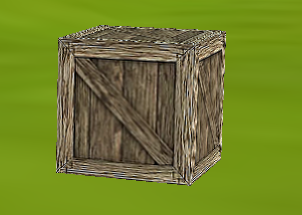
\includegraphics[width=90mm]{images/crates.png}
\caption{Box Obstacle}
\end{figure}

\begin{figure}[ht!]
\centering
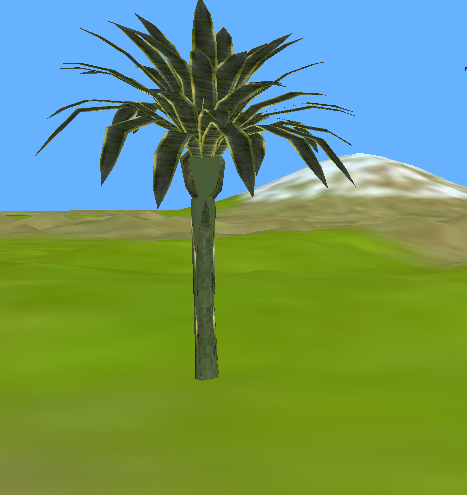
\includegraphics[width=90mm]{images/trees.png}
\caption{Tree Obstacle}
\end{figure}

\begin{figure}[ht!]
\centering
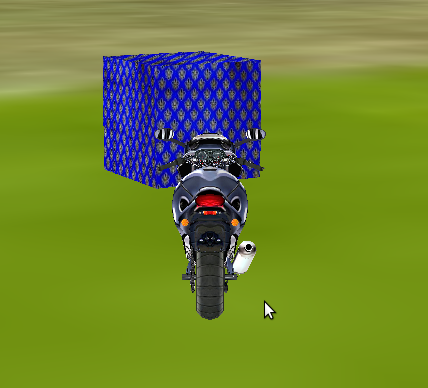
\includegraphics[width=90mm]{images/bonus.png}
\caption{Bonus Marker}
\end{figure}

\begin{figure}[ht!]
\centering
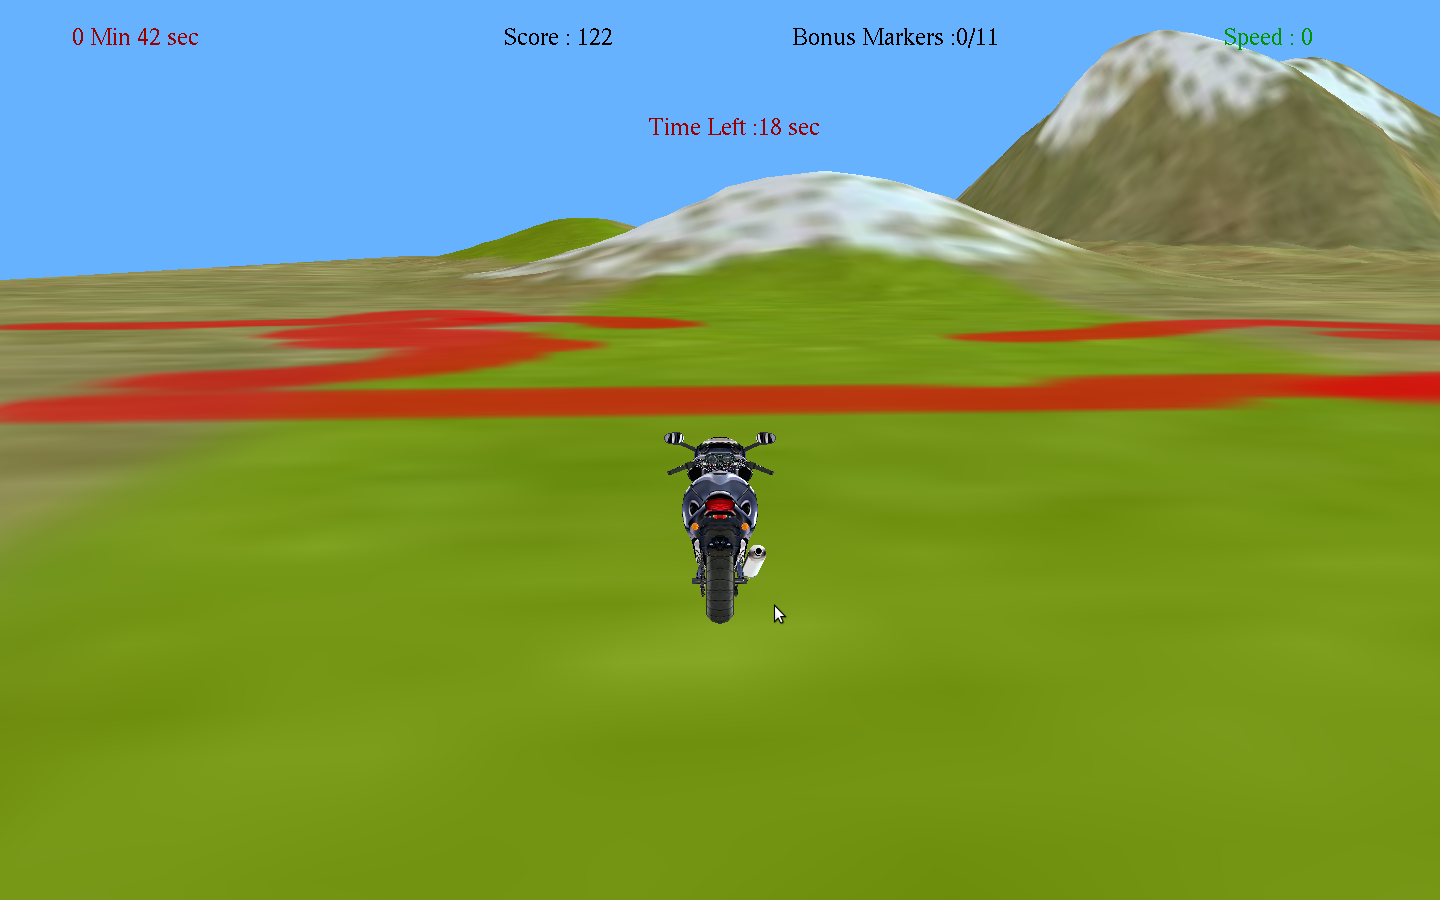
\includegraphics[width=90mm]{images/startLine.png}
\caption{Start Line}
\end{figure}

\end{flushleft}
\end{document}